\begin{frame}[t]{\secname}%{\subsecname}

\begin{columns}%[t]
  \begin{column}{0.37\textwidth}
    \begin{itemize}[noitemsep]
      \item Matrix identification
      \item Goal: Description of individual component material properties \& failure patterns before application in complex FRP structure
      \item LY564 bulk resin tensile tests ISO 527-2
      \item 1\textsuperscript{st} step: Discretization \& convergence study
      \begin{itemize}[noitemsep]
        \item LPS material model
        \item No surface correction
      \end{itemize}
    \end{itemize}
  \end{column}
  \begin{column}{0.18\textwidth}
    \begin{figure}
      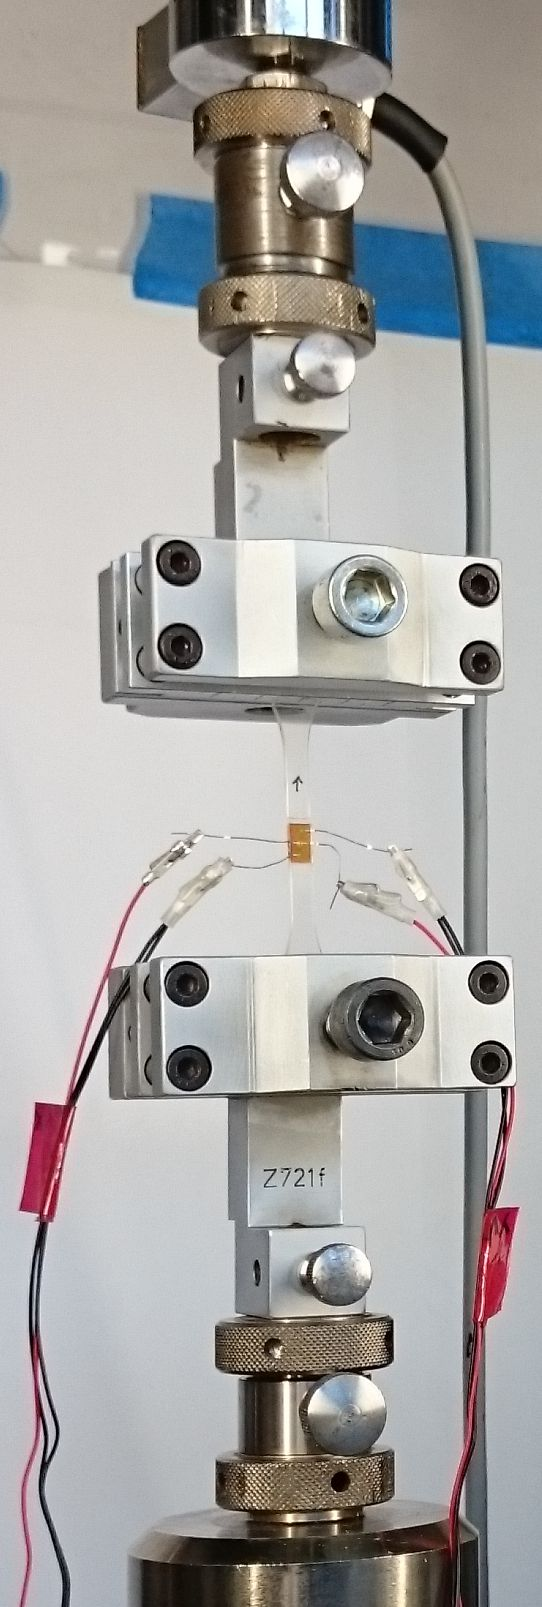
\includegraphics[width=\linewidth,height=0.75\textheight,keepaspectratio]{DSC_14001_c}
      \caption{Static test rig}
    \end{figure}
  \end{column}
  \begin{column}{0.44\textwidth}
%     \begin{figure}
    \begin{minipage}{\linewidth}
      \centering
      \tikzexternalenable
      \tikzsetnextfilename{Exp_Stress-Strain_LY564_1K-150-mittel}
      \begin{tikzpicture}
        \begin{axis}[
            axis lines=middle,
            width=\linewidth,
            height=0.5\textheight,
            font=\figurefontsize,
            xmin=0,
            xmin=0,
            xlabel={Strain $[\si{\percent}]$},
            ylabel={Stress $[\si{\mega\pascal}]$},
  %           x label style={at={(axis description cs:0.5,-0.15)},anchor=north},
  %           y label style={at={(axis description cs:-0.075,.5)},rotate=90,anchor=south},
            legend style={
              at={(1.0,0.55)},
              anchor=east,
              %font=\fontsize{4}{5}\selectfont,
              draw=none,
              fill=none,
              row sep=0.0pt,
              %inner sep=0.0,
            },
          ]
            %\addplot+[black,no marks] table[x=Strain, y=Stress] {\loadedtable};
            \addplot+[lightgray,dash dot,no marks] table[x=Strain, y=Stress, col sep=comma] {\materialpath/Data/Tests/Exp_Stress-Strain_LY564_1K-130-mittel.csv};
            \addlegendentry{Cure cycle 1}
            \addplot+[gray,solid,no marks] table[x=Strain, y=Stress, col sep=comma] {\materialpath/Data/Tests/Exp_Stress-Strain_LY564_1K-150-mittel.csv};
            \addlegendentry{Cure cycle 2}
            \addplot+[black,dashed,no marks] table[x=Strain, y=Stress, col sep=comma] {\materialpath/Data/Tests/Exp_Stress-Strain_LY564_3K-150-mittel.csv};
            \addlegendentry{Cure cycle 3}
        \end{axis}
      \end{tikzpicture}
      \tikzexternaldisable
      %\caption{Effective LY564 stress-strain curve}
      {\scriptsize Effective LY564 stress-strain curve}
    \end{minipage}\\
%     \end{figure}
    %\vfill
    \vspace{3ex}
    \begin{minipage}{\linewidth}
      \centering
%     \begin{figure}
      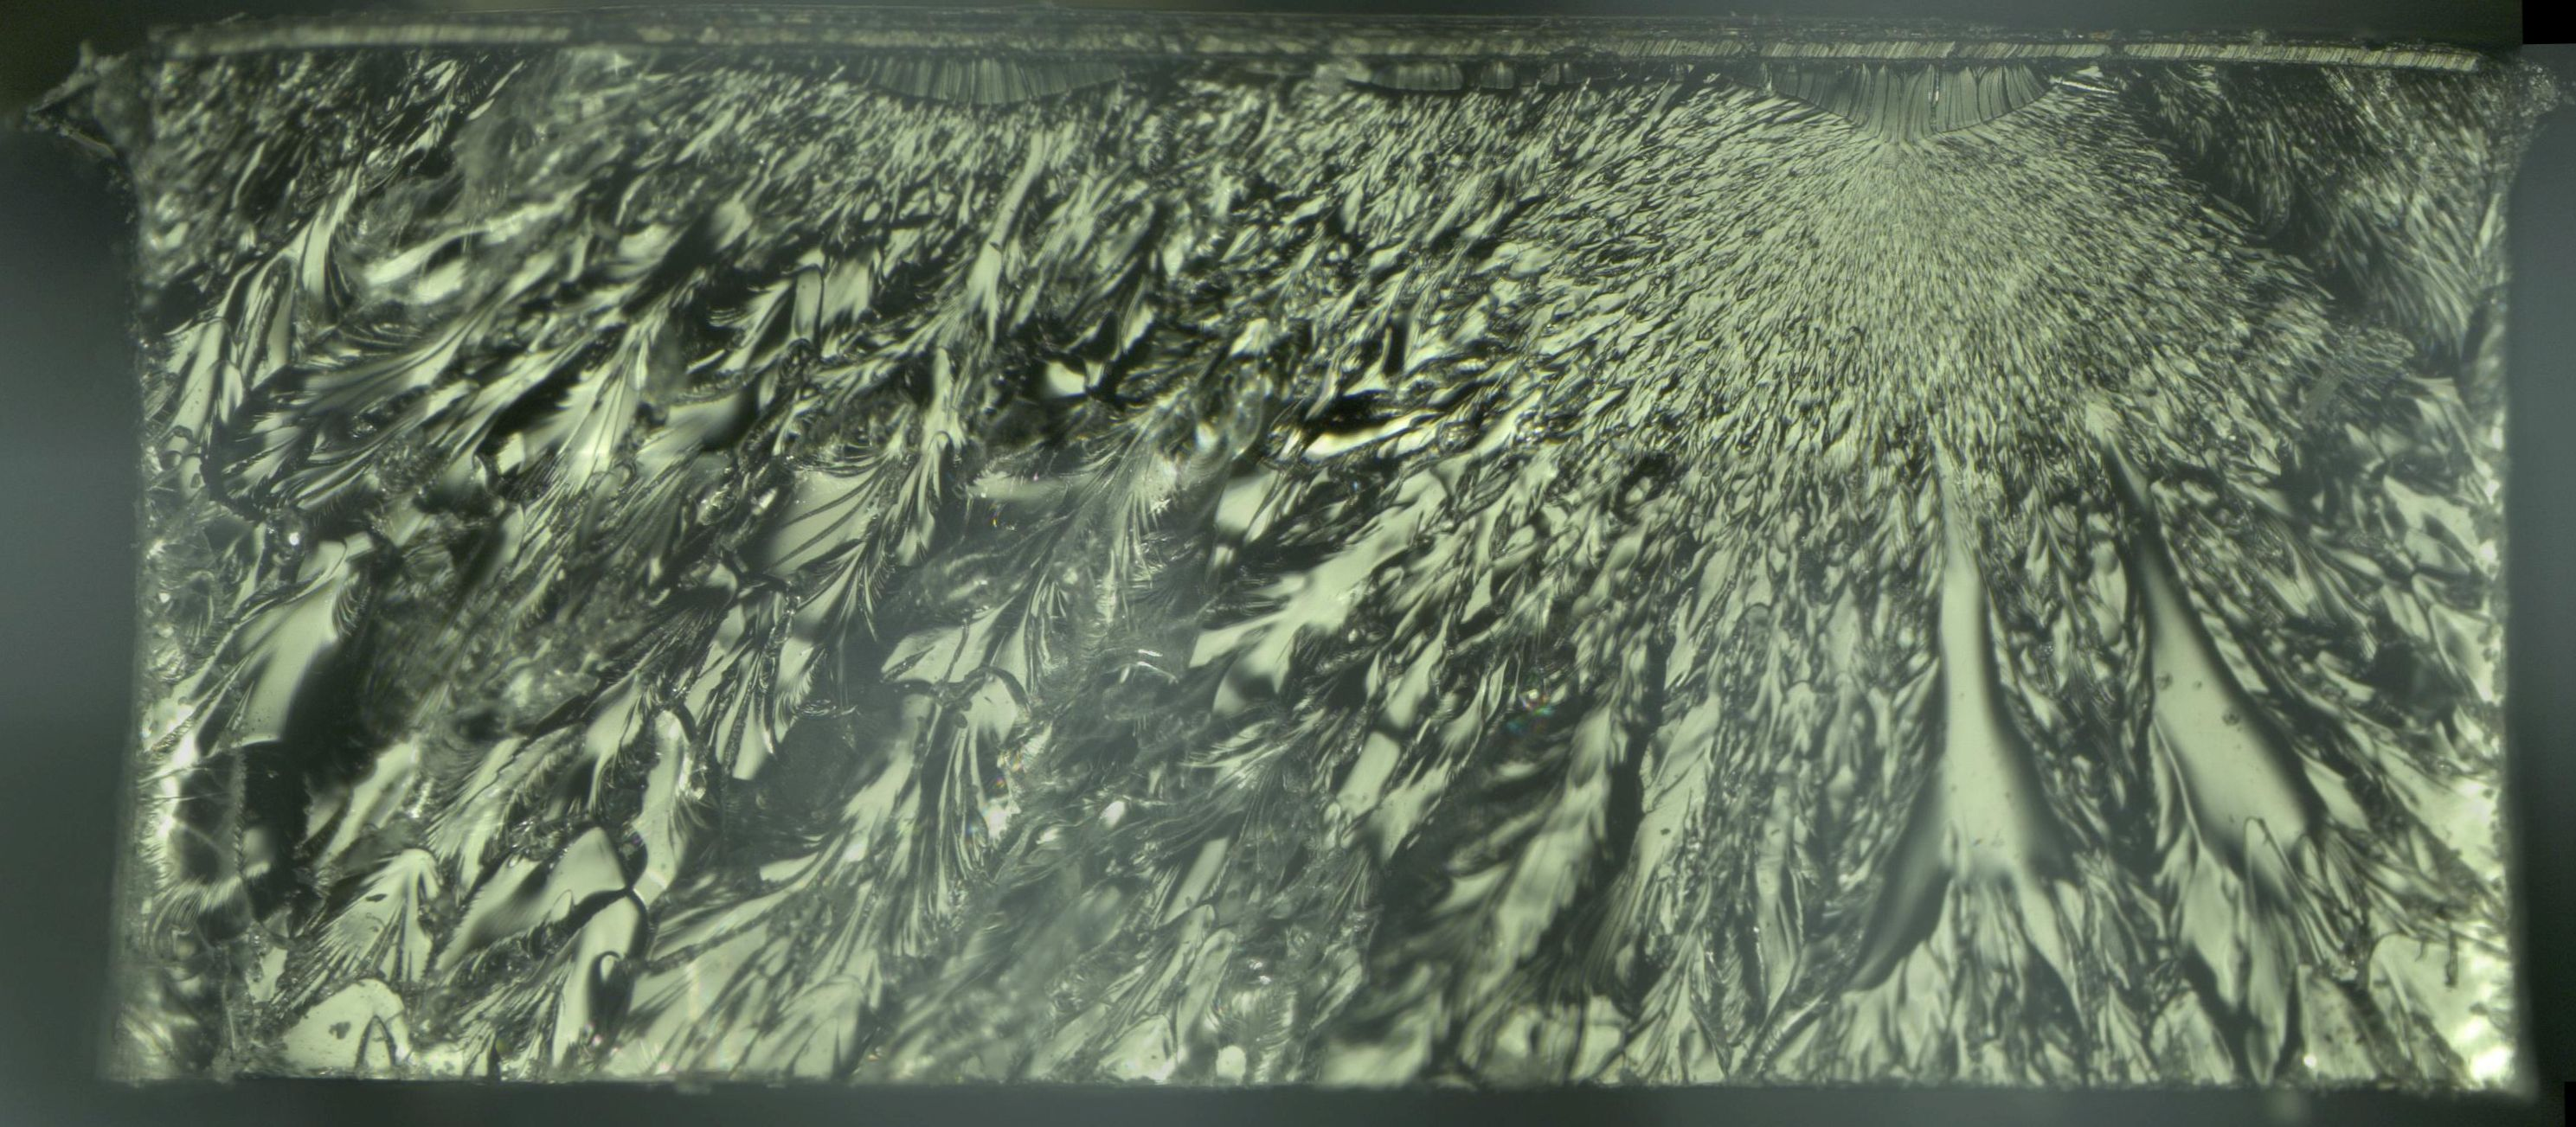
\includegraphics[width=\linewidth,height=0.3\textheight,keepaspectratio]{1K_150_02_c}\\
    %\caption{Fracture plane micrograph}
    {\scriptsize Fracture plane micrograph}
%     \end{figure}
    \end{minipage}

  \end{column}
\end{columns}
  
\end{frame}
